\chapter{Convergence numerical study}\label{ch:conv}

\section{Plate problems using known mixed finite elements}

\section{Non-standard discretization of flexible structures}


First of all we construct a family of finite elements capable of discretizing problem \eqref{eq:weak_mindlin}. Consider a regular triangulation $\mathcal{T}_h$ with elements $T$. The space of polynomials of order $k$ on a mesh cell is denoted by $P_k$. The following family of finite elements is conforming to the weak formulation \eqref{eq:weak_mindlin}
\begin{equation}\label{eq:CGDG}
\begin{aligned}
H_{h}^{1}(\Omega) &= \{w_h \in H^1(\Omega) \vert \ \forall T, \ w_h|_{T} \in P_{k} \}, \\
H_h^{\Grad}(\Omega, \bbR^2) &= \{ \bm{\theta}_h \in H^{\Grad}(\Omega, \bbR^2) \vert \ \forall T,\ \bm{\theta}_h|_{T} \in (P_{k})^2 \}, \\
L_h^2(\Omega, \mathbb{S}) &= \{ \bm{M}_h \in L^2(\Omega, \mathbb{S}) \vert \ \forall T, \bm{M}_h|_{T} \in (P_{k-1})^{2 \times 2}_{\text{sym}} \}, \\
L_h^2(\Omega, \bbR^2) &= \{\bm{q}_h \in L^2(\Omega, \bbR^2)  \vert \ \forall T,\ \bm{q}_h|_{T} \in (P_{k-1})^{2} \}, \\
\end{aligned}
\end{equation}
To approximate spaces $H_h^{1}(\Omega), \; H_h^{\Grad}(\Omega, \bbR^2)$ Lagrange polynomials of order $k$ are selected. For spaces $L_h^2(\Omega, \mathbb{S}), \; L_h^2(\Omega, \bbR^2)$ Discontinous Galerkin polynomials of order $k-1$ are employed. We use the acronym CGDG to denote this combination of elements
\[
\mathrm{CGDG} = \mathrm{CG} \times \mathrm{CG}(\bbR^2) \times \mathrm{DG}(\mathbb{S}) \times \mathrm{DG}(\bbR^2)
\]

This selection of finite elements can be seen as a standard discretization of the problem combined with a reduced integration of the stress tensor. For this reason, the following conjecture on the error estimates is proposed. 

\begin{conjecture}\label{conj:min}
	Assuming a smooth solution to problem~\eqref{eq:weak_mindlin}, the following error estimates hold 
	\begin{equation}
	\label{eq:errBEC}
	\begin{aligned}
	||e_w - e_w^h||_{L^{\infty}(H^1(\Omega))} &\lesssim h^{k}, \\
	||\bm{e}_\theta - \bm{e}_\theta^h||_{L^{\infty}(H^{\Grad}(\Omega, \bbR^2)} &\lesssim h^{k}, \\
	\end{aligned} \quad
	\begin{aligned}
	||\bm{E}_\kappa - \bm{E}_\kappa^h||_{L^{\infty}(L^2)} &\lesssim  h^{k}, \\
	||\bm{e}_\gamma - \bm{e}_\gamma^ h||_{L^{\infty}(L^2)} &\lesssim  h^{k}, \\
	\end{aligned} 
	\end{equation}
	where the notation $a \lesssim  b$ means $a \le C b$. The constant $C$ depends only on the true solution and on the final time.
\end{conjecture}

To validate the method first we test a finite element combinations on an analytic solution. Constructing an analytical solution for a vibrating Mindlin plate is far from trivial. Therefore, the solution for the static case \cite{veiga2013} is exploited. \\
\textbf{Step 1 } Consider a distributed static force given by 
\begin{equation*}
\begin{aligned}
f_s(x,y)=\frac{E_Y}{12 (1-\nu^2)} \{12 y(y-1)(5x^2-5x+1) \\
\times [2y^2(y-1)2+x(x-1)(5y^2-5y+1)] +12x(x-1)\\
\times (5y^2-5y+1)[2x^2(x-1)2+y(y-1)(5x^2-5x+1)]\}.
\end{aligned}
\end{equation*}
The static displacement and rotation are given by
\begin{align*}
w_s(x,y) &= \frac{1}{3} x^3(x-1)^3 y^3 (y-1)^3 -\frac{2 b^2}{5(1-\nu)}[y^3(y-1)^3 x(x-1)(5 x^2-5x+1). \\
\bm{\theta}_{s}(x,y) &= 
\begin{pmatrix}
y^3(y-1)^3 \ x^2 (x-1)^2 (2x-1) \\
x^3(x-1)^3 \ y^2 (y-1)^2 (2y-1) \\
\end{pmatrix}
\end{align*}
The static solution solves the following problem defined on the square domain $\Omega=(0,1)\times(0,1)$:
\begin{equation}
\begin{aligned}
0 &= \mathrm{div} \ \bm{q}_s + f_s , \\
0 &= \mathrm{Div} \bm{M}_s + \bm{q}_s, \\
\end{aligned} \qquad
\begin{aligned}
\bm{\mathcal{D}}_b^{-1} \bm{M}_s &= \mathrm{Grad} \ \bm{\theta}_s, \\
D_s^{-1} \bm{q}_s &= \mathrm{grad} \ w_s - \bm{\theta}_s. \\
\end{aligned}
\end{equation}
\textbf{Step 2 } Given the linear nature of the system a solution for the dynamic problem is found by multiplying the static solution by a time dependent term. For simplicity a sinus function is chosen
\[
w_d(x,y,t) = w_s(x,y) \sin(t), \quad \bm{\theta}_d(x,y,t) = \bm\theta_s(x,y) \sin(t).
\]
For the port-Hamiltonian system velocities are needed
\[
e_w^\text{ex}(x,y,t) = w_s(x,y) \cos(t), \quad \bm{e}_\theta^\text{ex}(x,y,t) = \bm\theta_s(x,y) \cos(t).
\]
The momenta and shear force are then defined by
\[
\bm{M}_d = \bm{E}_\kappa^\text{ex} =  \bm{\mathcal{D}}_b \ \mathrm{Grad} \ \bm{\theta}_d, \quad \bm{q}_d = \bm{e}_\gamma^\text{ex} = D_s(\mathrm{grad} \ w_d - \bm{\theta}_d)
\]
\textbf{Step 3 } Appropriate forcing terms have to be introduced (i.e. $f, \bm{\tau}$ in \eqref{eq:clMin}). The force and torque in the dynamical case become
\begin{equation*}
f_d = f_s \sin(t) + \rho b \partial_{tt} w_d, \qquad \bm{\tau}_d = \frac{\rho b^3}{12} \partial_{tt} \bm{\theta}_d.
\end{equation*}
Variables $(e_w^\text{ex}, \bm{e}_\theta^\text{ex}, \bm{E}_\kappa^\text{ex}, \bm{e}_\gamma^\text{ex})$ under excitations $(f_d, \bm{\tau}_d)$ solve problem~\eqref{eq:pHdyn_Min1}. The solution being smooth, the conjectured error estimates \ref{conj:min} should hold. The numerical values of the physical parameters are reported in Table \ref{tab:parMin}.  To integrate the equations in time a Crank-Nicholson scheme has been used. The time step is set to $\Delta t = h/10$ to have a lower impact of the time discretization error with respect to the spatial error. The final time is set to one $t_f = 1 [\textrm{s}]$.

\begin{table}[htb]
	\centering
	\begin{tabular}{ccccc}
		\hline 
		\multicolumn{5}{c}{Plate parameters} \\ 
		\hline 
		$E$ & $\rho$ & $\nu$ & $k$ & $h$ \\
		1 $[\textrm{Pa}]$ & $1\; [\textrm{kg}/\textrm{m}^3]$ & 0.3 & 5/6 & 0.1 $[\textrm{m}]$\\ 
		\hline 
	\end{tabular} 
	\captionsetup{width=0.95\linewidth}
	\vspace{1mm}
	\captionof{table}{Physical parameters for the Mindlin plate.}
	\label{tab:parMin}
\end{table}

\begin{table}[htb]
	\centering
	\begin{tabular}{ccccccccc}
		\hline 
		\multirow{2}{*}{$\frac{1}{h}$} & \multicolumn{2}{c}{$||e_w - e_w^h||_{L^{\infty}(H^1)}$}    & \multicolumn{2}{c}{$||\bm{e}_\theta - \bm{e}_\theta^h||_{L^{\infty}(H^{\Grad})}$} & \multicolumn{2}{c}{$||\bm{E}_\kappa - \bm{E}_\kappa^h||_{L^{\infty}(L^2)}$} & \multicolumn{2}{c}{$||\bm{e}_\gamma - \bm{e}_\gamma^ h||_{L^{\infty}(L^2)}$}   \\ 
		& Error & Order  & Error & Order  & Error & Order  & Error & Order   \\ 
		\hline 
		8  & 7.30e-05 & ---  & 5.52e-04 & ---  & 3.99e-08 & ---  & 9.02e-07 & --- \\ 
		16 & 3.13e-05 & 1.22 & 2.26e-04 & 1.28 & 1.88e-08 & 1.08 & 5.47e-07 & 0.72\\ 
		32 & 1.57e-05 & 0.99 & 1.11e-04 & 1.02 & 8.84e-09 & 1.09 & 2.94e-07 & 0.89\\ 
		64 & 7.87e-06 & 0.99 & 5.57e-05 & 0.99 & 4.31e-09 & 1.03 & 1.50e-07 & 0.97\\ 
		128& 3.94e-06 & 0.99 & 2.78e-05 & 0.99 & 2.14e-09 & 1.01 & 7.55e-08 & 0.99\\ 
		\hline 
	\end{tabular} 
	\captionsetup{width=0.95\linewidth}
	\vspace{1mm}
	\captionof{table}{Mindlin plate convergence result $k=1$.}
	\label{tab:resmin_k1}
\end{table}


\begin{table}[htb]
	\centering
	\begin{tabular}{ccccccccc}
		\hline 
		\multirow{2}{*}{$\frac{1}{h}$} & \multicolumn{2}{c}{$||e_w - e_w^h||_{L^{\infty}(H^1)}$}    & \multicolumn{2}{c}{$||\bm{e}_\theta - \bm{e}_\theta^h||_{L^{\infty}(H^{\Grad})}$} & \multicolumn{2}{c}{$||\bm{E}_\kappa - \bm{E}_\kappa^h||_{L^{\infty}(L^2)}$} & \multicolumn{2}{c}{$||\bm{e}_\gamma - \bm{e}_\gamma^ h||_{L^{\infty}(L^2)}$}   \\
		& Error & Order  & Error & Order  & Error & Order  & Error & Order   \\ 
		\hline 
		8  & 9.78e-06 & ---  & 1.04e-04 & ---  & 7.30e-09 & ---  & 1.77e-07 & --- \\ 
		16 & 2.53e-06 & 1.95 & 2.49e-05 & 2.07 & 1.85e-09 & 1.97 & 4.93e-08 & 1.84\\ 
		32 & 6.35e-07 & 1.99 & 6.06e-06 & 2.04 & 4.63e-10 & 1.99 & 1.27e-08 & 1.95\\ 
		64 & 1.58e-07 & 1.99 & 1.50e-06 & 2.01 & 1.15e-10 & 2.00 & 3.21e-09 & 1.98\\ 
		128& 3.97e-08 & 2.00 & 3.74e-07 & 2.00 & 2.89e-11 & 2.00 & 8.06e-10 & 1.99\\ 
		\hline 
	\end{tabular} 
	\captionsetup{width=0.95\linewidth}
	\vspace{1mm}
	\captionof{table}{Mindlin plate convergence result $k=2$.}
	\label{tab:resmin_k2}
\end{table}


\begin{table}[htb]
	\centering
	\begin{tabular}{ccccccccc}
		\hline 
		\multirow{2}{*}{$\frac{1}{h}$} & \multicolumn{2}{c}{$||e_w - e_w^h||_{L^{\infty}(H^1)}$}    & \multicolumn{2}{c}{$||\bm{e}_\theta - \bm{e}_\theta^h||_{L^{\infty}(H^{\Grad})}$} & \multicolumn{2}{c}{$||\bm{E}_\kappa - \bm{E}_\kappa^h||_{L^{\infty}(L^2)}$} & \multicolumn{2}{c}{$||\bm{e}_\gamma - \bm{e}_\gamma^ h||_{L^{\infty}(L^2)}$}   \\
		& Error & Order  & Error & Order  & Error & Order  & Error & Order   \\ 
		\hline 
		4  & 1.38e-06 & ---  & 1.24e-05 & ---  & 8.24e-10 & ---  & 2.24e-08 & --- \\ 
		8  & 1.79e-07 & 2.94 & 1.51e-06 & 3.03 & 1.03e-10 & 2.99 & 2.90e-09 & 2.94\\ 
		16 & 2.26e-08 & 2.98 & 1.88e-07 & 3.00 & 1.28e-11 & 3.00 & 3.64e-10 & 2.99\\ 
		32 & 2.83e-09 & 2.99 & 2.36e-08 & 2.99 & 1.60e-12 & 3.00 & 4.54e-11 & 3.00\\ 
		64 & 3.54e-10 & 2.99 & 2.95e-09 & 2.99 & 2.00e-13 & 3.00 & 5.67e-12 & 3.00\\ 
		\hline 
	\end{tabular} 
	\captionsetup{width=0.95\linewidth}
	\vspace{1mm}
	\captionof{table}{Mindlin plate convergence result $k=3$.}
	\label{tab:resmin_k3}
\end{table}

\begin{figure}[t]%
	\centering
	\subfloat[][$L^\infty_{\Delta t} ( H^1(\Omega))$ error for $e_w$]{%
		\label{fig:errCGDG1}%
		\includegraphics[width=0.4\columnwidth]{part_3/CCCC_CGDG__vel.eps}}%
	\hspace{8pt}%
	\subfloat[][$L^\infty_{\Delta t} (H^{\Grad}(\Omega, \bbR^2))$ error for $\bm{e}_\theta$]{%
		\label{fig:errCGDG2}%
		\includegraphics[width=0.4\columnwidth]{part_3/CCCC_CGDG__om.eps}} \\
	\subfloat[][$L^\infty_{\Delta t} (L^2(\Omega, \mathbb{S}))$ error for $\bm{E}_\kappa$]{%
		\label{fig:errCGDG3}%
		\includegraphics[width=0.4\columnwidth]{part_3/CCCC_CGDG__sig.eps}}%
	\hspace{8pt}%
	\subfloat[][$L^\infty_{\Delta t} (L^2)$ error for $\bm{e}_\gamma$]{%
		\label{fig:errCGDG4}%
		\includegraphics[width=0.4\columnwidth]{part_3/CCCC_CGDG__q.eps}}%
	\caption[errorBEC]{Error for the Mindlin plate using the CGDG elements}%
	\label{fig:errorBEC}%
\end{figure}
